\chapter{Dataset analysis and preparation}\label{sec:data-ana}

The dataset used in this thesis is the Indoor Location \& Navigation from kaggle\cite{kaggle} which was part of a competition of Microsoft Research in 2021\cite{IndoorLocationNavigation}.
The data was recorded in shopping malls by the company XYZ\(^{10}\) and was provided by Microsoft Research for this competition.
The goal for the competition was, given a site-path file, predict the floor and waypoint locations at a timestamp given in the submission files.
In the following, the dataset and data will be analyzed.


\section{Components of the dataset}\label{sec:data}
As noted in the kaggle notebook ``Indoor Navigation: Complete Data Understanding'' \cite{IndoorNavigationUnderstanding} the data consists of 3 parts:

\begin{itemize}
    \item a train folder with train path files, organized by site and floor
    \item a test folder with test path files, organized by site and floor but without waypoint data
    \item a metadata folder with floor metadata, organized by site and floor, which includes floor images, further information and a geojson map
\end{itemize}

The train folder contains 204 subfolders, which represent each site where the data was recorded.
In each site folder are a minimum of one and a maximum of twelve subfolders, which represent the floors of the site, the median is 5 floors.
Overall there are 26,925 files each containing the movement of one person for a specific site and floor.
Per floor there are between one and 284 files with a median of 14.
The floor F1 of site \begin{CJK*}{UTF8}{gbsn}银泰城(城西店)\end{CJK*} which was hashed as ``5d27075f03f801723c2e360f'' in the train folder of the competition, has the most files.

For this thesis, the submission files as well as the test folder will not be used, because our goal is not to predict the floor and site name for a certain timestamp, but to predict the \ac{bssid} to which a device may connect next.
Therefore, we will not analyze the content of these folders in more detail.

\section{File structure}\label{sec:file-structure}

Each file in each floor folder is a \textbf{.txt} file. 
The first two lines and the last are denoted with ``\#''.
The first contains the start time of the recording, the second site information SiteID as hash, SiteName, FloorId as hash and FloorName.
The last line contains the end time of the recording.
The main part of the data consists of the collected data. 
Each line contains a UNIX timestamp in milliseconds, followed by a data type and the data itself, which are all separated by a tabulator.
The GitHub repository of the competition\cite{GitHubComp} shows that the data type in the second column followed by its data can be one of the following:

\setlist[enumerate]{label=(\arabic*)}
\begin{enumerate}
    \item\label{type:acce} TYPE\_ACCELEROMETER with x, y and z acceleration and an accuracy value
    \item\label{type:mag} TYPE\_MAGNETIC\_FIELD with x, y and z magnetic field and an accuracy value
    \item\label{type:gyro} TYPE\_GYROSCOPE with x, y and z gyroscope and an accuracy value
    \item\label{type:rot} TYPE\_ROTATION\_VECTOR with x, y and z rotation vector and an accuracy value
    \item\label{type:mag_u} TYPE\_MAGNETIC\_FIELD\_UNCALIBRATED with x, y and z magnetic field and an accuracy value
    \item\label{type:gyro_u} TYPE\_GYROSCOPE\_UNCALIBRATED with x, y and z gyroscope and an accuracy value
    \item\label{type:acce_u} TYPE\_ACCELEROMETER\_UNCALIBRATED with x, y and z acceleration and an accuracy value
    \item\label{type:wifi} TYPE\_WIFI with \ac{ssid}, \ac{bssid}, \ac{rssi}, frequency, and last seen timestamp of the access point. The SSID and BSSID are hashed.
    \item\label{type:beacon} TYPE\_BEACON with \ac{uuid}, \ac{MajorID}, \ac{MinorID}, \ac{TxPower}, \ac{rssi}, distance to the device measured by the beacon, \ac{mac} address and a timestamp as padding data. The MajorID and MinorID are hashed.
    \item\label{type:way} TYPE\_WAYPOINT with x and y coordinates which are the ground truth location labeled by the surveyor
\end{enumerate}

\lstset{
    basicstyle=\scriptsize\ttfamily,
    breaklines=true,
    escapeinside={(*@}{@*)},
}

\begin{lstlisting}[caption={A snippet from the dataset of a file of the floor F4 of the site with the ID 5d27099303f801723c32364d},label={lst:dataset},captionpos=b]
    #	startTime:1571462193934
    #	SiteID:5d27099303f801723c32364d	SiteName:(*@\begin{CJK*}{UTF8}{gbsn}银泰百货(庆春店)\end{CJK*}@*) FloorId:5d27099303f801723c323650	FloorName:4F
    1571462193944	TYPE_WAYPOINT	57.885998	69.501526
    1571462194071	TYPE_ACCELEROMETER	-0.95254517	0.7944031	8.928757	2
    1571462194071	TYPE_MAGNETIC_FIELD	-25.65918	-4.4784546	-28.201294	3
    1571462194071	TYPE_GYROSCOPE	-0.22373962	-0.07733154	-0.16847229	3
    1571462194071	TYPE_ROTATION_VECTOR	0.04186145	-0.02101801	-0.72491926	3
    1571462194071	TYPE_MAGNETIC_FIELD_UNCALIBRATED	-4.8568726	10.406494	-387.44965	20.802307	14.884949	-359.24835	3
    1571462194071	TYPE_GYROSCOPE_UNCALIBRATED	-0.22218323	-0.068359375	-0.1628418	0.0026245117	9.765625E-4	-7.6293945E-4	3
    1571462194071	TYPE_ACCELEROMETER_UNCALIBRATED	-0.95254517	0.7944031	8.928757	0.0	0.0	0.0	3
    ...
    1571462194883	TYPE_WIFI	b06c4e327882fab58dfa93ea85ca373a54e887b5	9f967858afcbb907af6e5adef766c7e7b936ef07	-63	2462	1571462190744
    1571462194883	TYPE_WIFI	8204870beb9d02995dab3f08aad97af5eab723cc	0413b35df78fc865af15b4721d5aeb33ff57da45	-64	2447	1571462188686
    ...
    1571462194020	TYPE_BEACON	07efd69e3167537492f0ead89fb2779633b04949	b6589fc6ab0dc82cf12099d1c2d40ab994e8410c	76e907e391ad1856762f70538b0fd13111ba68cd	-57	-71	5.002991815535578	1b7e1594febd760b00f1a7984e470867616cee4e	1571462194020
    ...
    #	endTime:1571462195976
\end{lstlisting}

Each file contains a different amount of waypoints and sensor data.
The first and last data type in each file is a \ref{type:way}.
Lines with types from \ref{type:acce} to \ref{type:acce_u} occur every 20 ms and are measured at the same time.
\ref{type:wifi} occurs about every 1800-2200 ms.
\ref{type:way} data is not evenly distributed.
An assumption for this is, that the recording of the waypoint data is triggered by an exterior event, e.g. a button press.
As seen in \cref{lst:dataset}, the data are measured separately from each other, so there are no combinations of the data types.

A prediction of the next \ac{bssid} will only work per site, due to the different architectures of the sites.
Still, prediction could be difficult for a whole site, because the \acp{ap} are different on each floor which may result in many \acp{ap} for the prediction.
To get better results in the prediction, we will focus on a single floor of a site.
The \cref{tab:data_summary} shows an analysis of the site with the most files for a single floor.
% \subsection{Analysis of floor with most files}
\begin{table}[h]
    \centering
    \begin{tabular}{|l|l|}
    \hline
    \textbf{Information} & \textbf{Value} \\ \hline
    Total data points & 7,157,081 \\ \hline
    Average data points per file & 25,201 \\ \hline
    Number of waypoints & 2,027 \\ \hline
    Lines of each \ref{type:acce} to \ref{type:acce_u} data & 746,689 \\ \hline
    Lines of \ac{wifi} data & 1,862,044 \\ \hline
    Lines of beacon data & 66,187 \\ \hline
    Number of \acp{bssid} & 4,795 \\ \hline
    Number of \acp{ap} & 4,795 \\ \hline
    Number of \acp{ssid} & 1,421 \\ \hline
    \ac{rssi} range & -93 to -13 dBm \\ \hline
    \end{tabular}
\caption{Summary of data for F1 of site \begin{CJK*}{UTF8}{gbsn}银泰城(城西店)\end{CJK*}}
\label{tab:data_summary}
\end{table}

% To gain more information on the data, we will analyze the files in F1 of site \begin{CJK*}{UTF8}{gbsn}银泰城(城西店)\end{CJK*}.
% We have 7,157,081 data points distributed in 284 files, which are 25,201 data points per file on average.
% 2027 of those are waypoints.
% 746,689 lines are accelerometer and uncalibrated, magnetic field and uncalibrated, gyroscope and uncalibrated, and rotation vector.
% 1,862,044 lines are \ac{wifi} and 66,187 lines are beacon data.
% A visualization of the waypoints can be seen in \cref{fig:vis-wo-interpolated}.
% On this floor are 4795 \acp{bssid}, so 4795 \acp{ap}, which emit 1,421 \acp{ssid}.
% The \ac{rssi} ranges from -93 dBm to -13 dBm.

\begin{figure}
    \centering
\includegraphics[scale=0.435]{images/whole_floor_visualization_wo_interpolated.png}
\caption[]{Visualization of the waypoints for SiteName: \begin{CJK*}{UTF8}{gbsn}银泰城(城西店)\end{CJK*}}
\label{fig:vis-wo-interpolated}
\end{figure}


\section{Improvement on data for an ML model}\label{sec:improvement-on-data-for-an-ml-model}

As seen in previous sections, a location for the time of \(TYPE\_WIFI\) data points is not provided.
Between \(TYPE\_WAYPOINT\) and \(TYPE\_WIFI\) data further human movement may have occurred.
However, they can be combined using linear interpolation, as seen in \cref{fig:interpolation}.
\begin{figure}
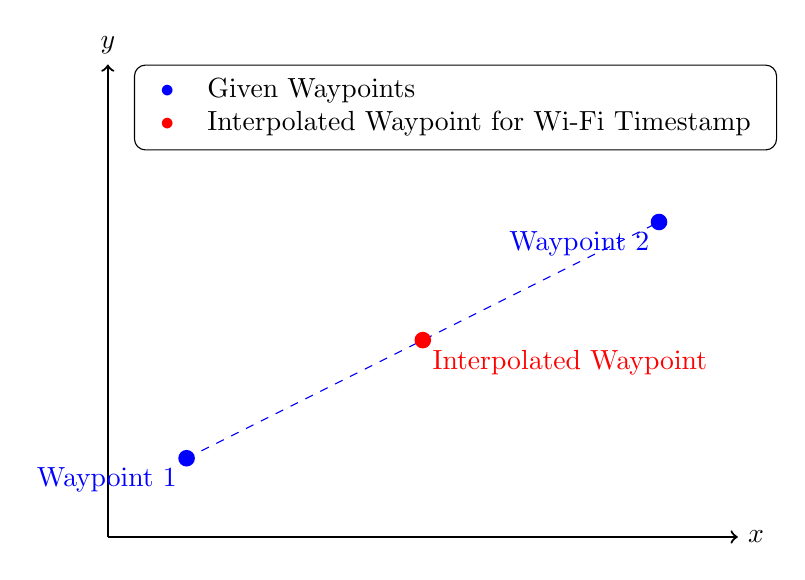
\begin{tikzpicture}
    % Axis
    \draw[->, thick] (0,0) -- (8,0) node[right] {$x$};
    \draw[->, thick] (0,0) -- (0,6) node[above] {$y$};

    % Given Waypoints (e.g., from the waypoints data)
    \fill[blue] (1,1) circle (3pt) node[below left] {Waypoint 1};
    \fill[blue] (7,4) circle (3pt) node[below left] {Waypoint 2};
    \draw[dashed, blue] (1,1) -- (7,4);

    % Interpolated Points (e.g., for wifi_timestamps)
    \fill[red] (4,2.5) circle (3pt) node[below right] {Interpolated Waypoint};

    % Legend
    \node[draw, rectangle, rounded corners, fill=white, anchor=north east] at (8.5,6) {
        \begin{tabular}{c l}
        \color{blue} $\bullet$ & Given Waypoints \\
        \color{red} $\bullet$ & Interpolated Waypoint for Wi-Fi Timestamp \\
        \end{tabular}
    };
\end{tikzpicture}
\caption{Visualization of linear interpolation for \ac{wifi} timestamps based on given waypoints. The blue points represent the original waypoints, while the red points show the interpolated positions for specific \ac{wifi}}
\label{fig:interpolation}
\end{figure}

Thus, \(TYPE\_WAYPOINT\) and \(TYPE\_WIFI\) are combined to get a location for the \ac{wifi} data point.
The interpolation results in 6549 waypoints which is 3 times more than the original amount of waypoints, as seen in \cref{fig:vis-interpolated}.
\begin{figure}
    \centering
\includegraphics[scale=0.435]{images/whole_floor_visualization_interpolated.png}
\caption[]{Visualization of the interpolated waypoints for SiteName: \begin{CJK*}{UTF8}{gbsn}银泰城(城西店)\end{CJK*}}
\label{fig:vis-interpolated}
\end{figure}
Furthermore, we will also interpolate \(TYPE\_ACCELEROMETER\) to improve the predictions.
Now a multivariate time series is interpolated out of the original data, which will be used for the machine learning model.
A further interpolation is possible, but we will focus on a simpler multivariate time series. %because?


\section{Peculiarities of the data}\label{sec:special-cases}
Further analysis of the dataset revealed some peculiarities, which are described in the following.

The data is collected by different devices, at different timestamps and days.
A problem for the ML could be, that the waypoint data were measured irregularly.
\begin{itemize}
    \item As in \cref{fig:vis-wo-interpolated} some waypoints seem to be very distant from the next one
    \item \cref{lst:metric-diff} shows the top 10 pairs of waypoints with the most significant metric differences
    \item if points are more than 10 meters apart, we will define them as ``to apart from each other''
    \item split up the data where the distance between two points is more than 10 meters
    \item result: 123 files, with interpolation
\end{itemize}

\begin{lstlisting}[caption={Top 10 pairs with the most significant metric differences},label={lst:metric-diff},captionpos=b]
    1. Point 1: (247.96523998265695, 168.7631635050295), Point 2: (117.92375106521739, 51.997759545341616), Metric Difference: 174.77113148839442
    2. Point 1: (98.66346, 127.5971), Point 2: (258.75049789436116, 181.23350740899357), Metric Difference: 168.83342057049657
    3. Point 1: (189.58672, 71.454666), Point 2: (89.73448203762376, 102.255128190099), Metric Difference: 104.49467879858156
    4. Point 1: (223.49295, 145.0939), Point 2: (174.26284532732006, 78.86335505811792), Metric Difference: 82.52325908119289
    5. Point 1: (34.864815, 35.45561), Point 2: (33.284438514193546, 110.76117936967742), Metric Difference: 75.32215057954856
    6. Point 1: (50.31085719185683, 92.03105531572366), Point 2: (114.97229034709193, 123.04521228267667), Metric Difference: 71.71456525741291
    7. Point 1: (150.91972285390713, 145.15169976783693), Point 2: (222.23440919809525, 146.11043967333333), Metric Difference: 71.32113060360388
    8. Point 1: (64.64140228107132, 25.345204272946134), Point 2: (34.47475562023909, 84.44615420072283), Metric Difference: 66.35471990088624
    9. Point 1: (56.83799274253731, 74.52090035349569), Point 2: (94.43750948519768, 125.97292215289488), Metric Difference: 63.72624425248555
    10. Point 1: (172.3439286324042, 56.200716101045295), Point 2: (212.4478039192399, 99.33967479470648), Metric Difference: 58.90068395354572
\end{lstlisting}

